\section{Introduction}
\label{sec:intro}

\begin{figure}[!t]
	\centering
	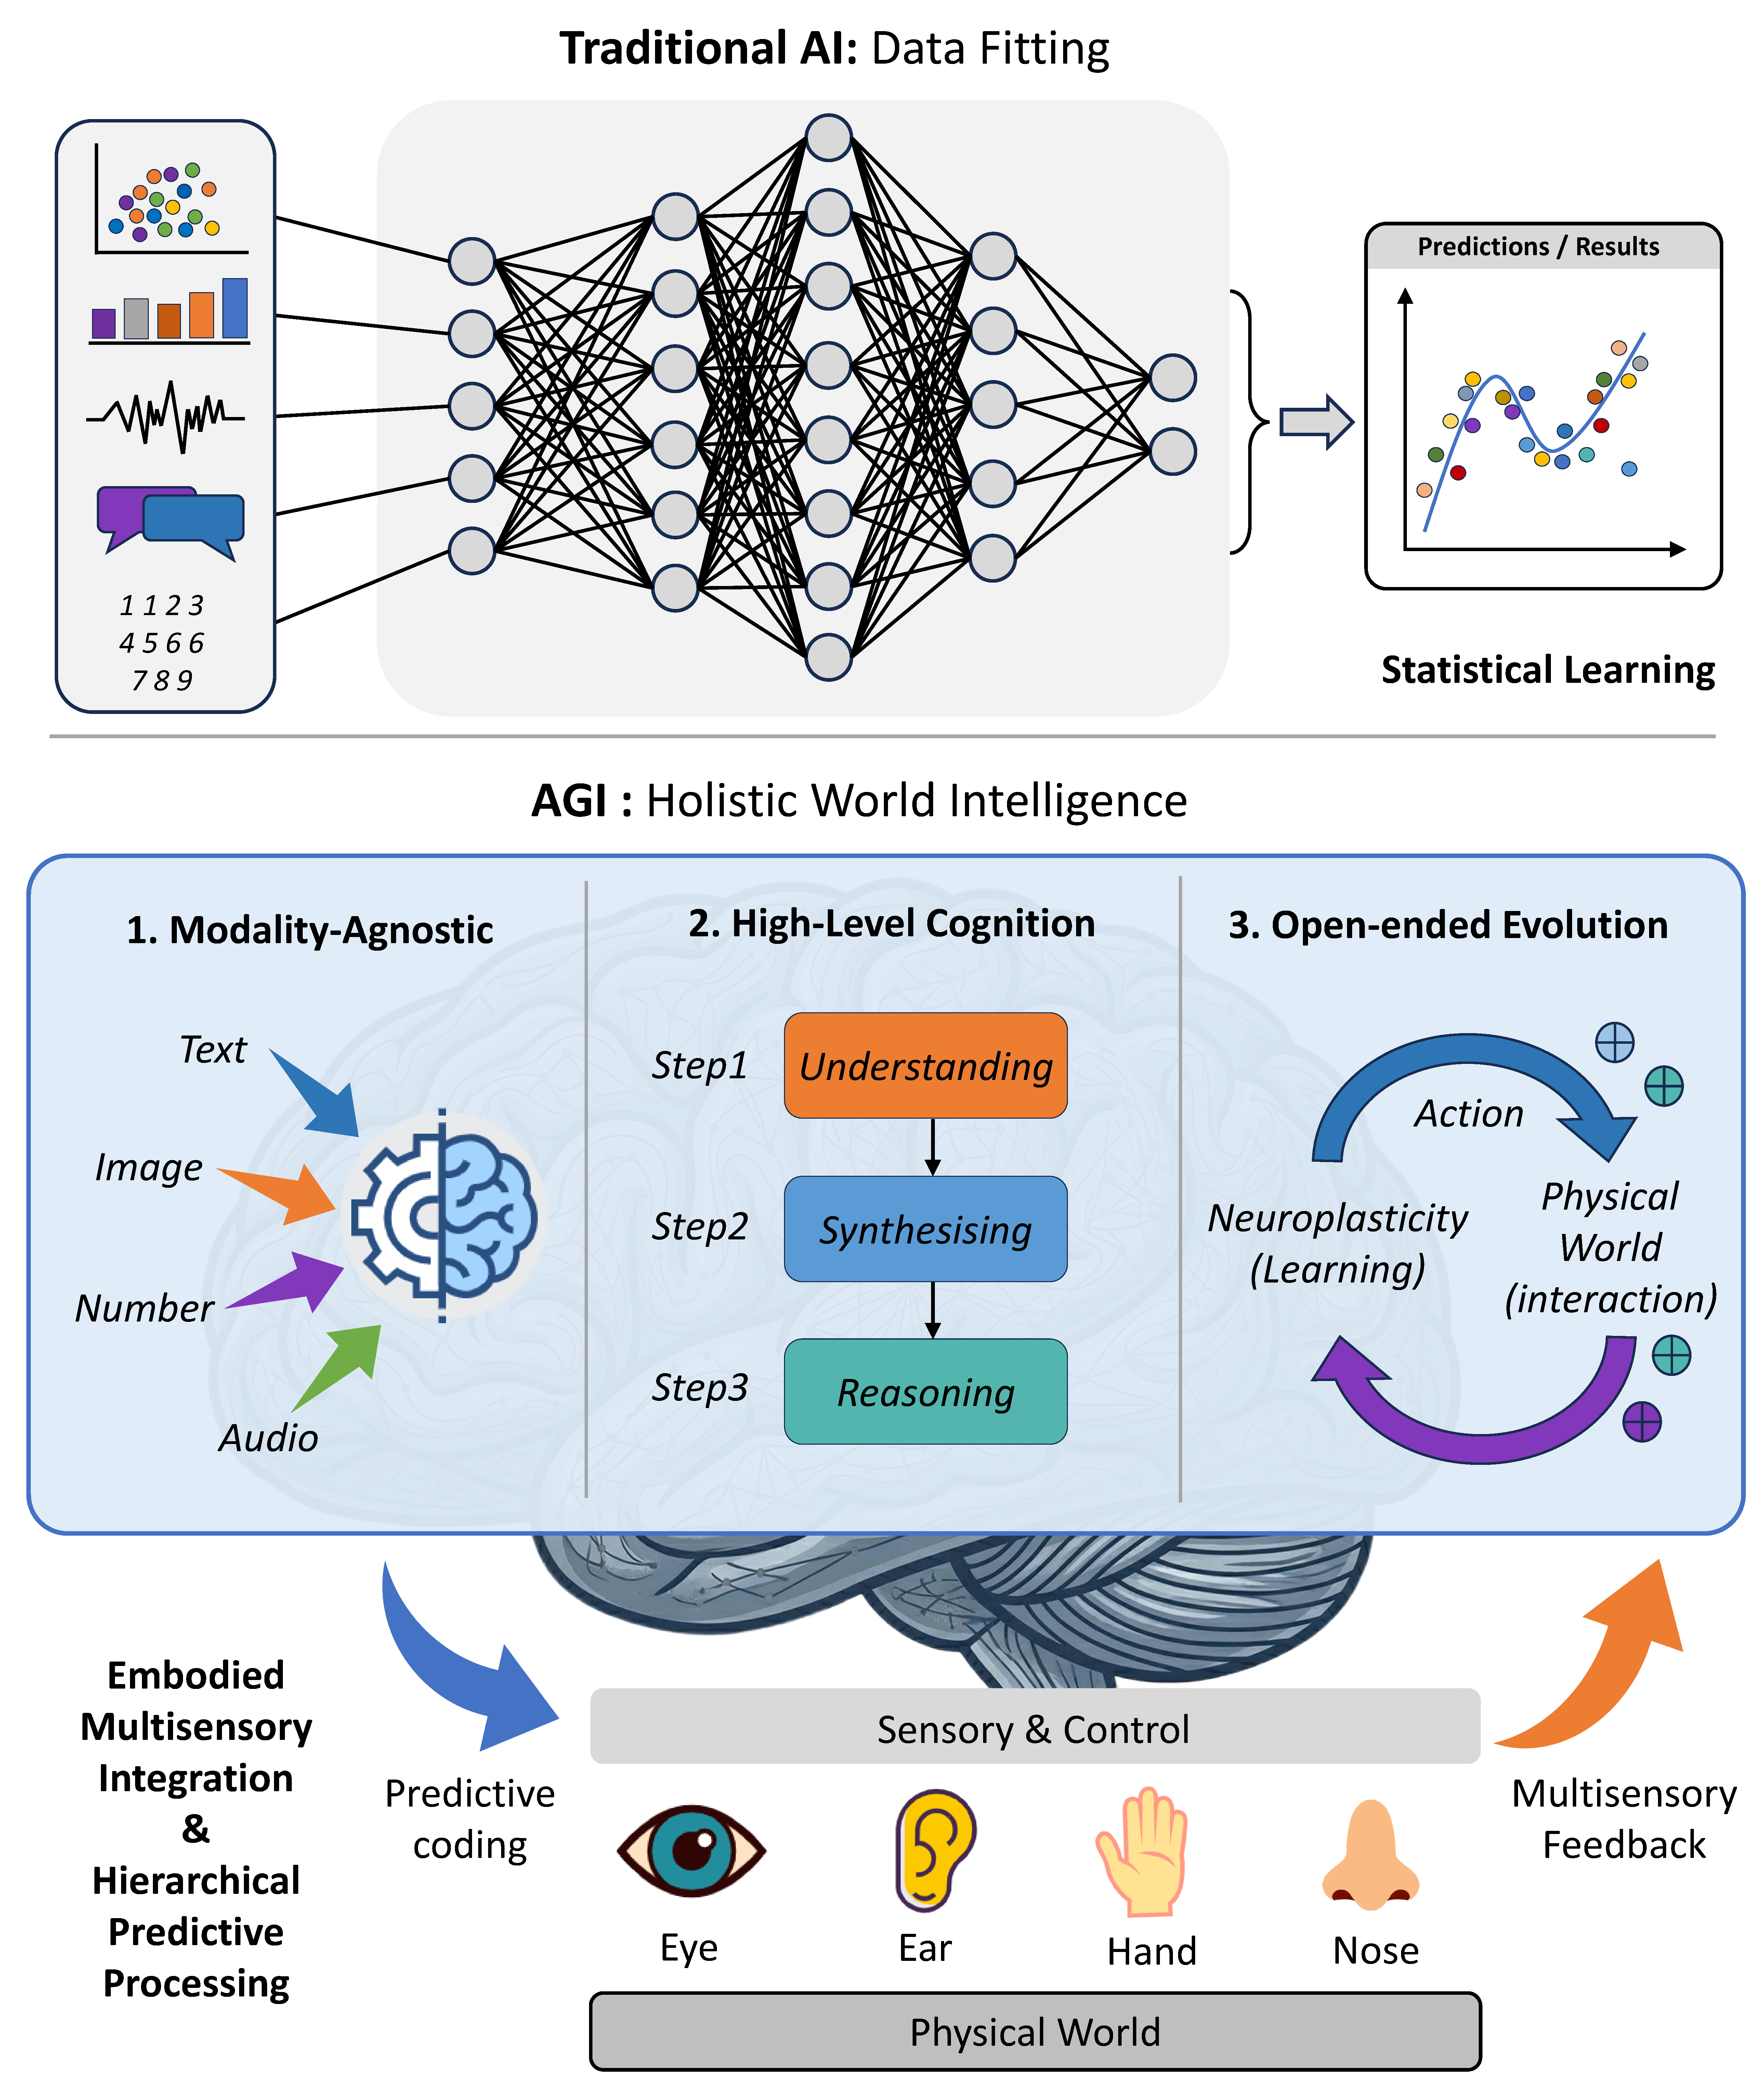
\includegraphics[scale=0.1]{figure/figure1.pdf}
    \vspace{-3mm}
	\caption{The Paradigm Shift from Traditional Statistical Data Fitting to Holistic World Intelligence (HWI) for AGI. }
    \vspace{-5mm}
	\label{figure1}
\end{figure}

\begin{figure*}[!t]
	\centering
	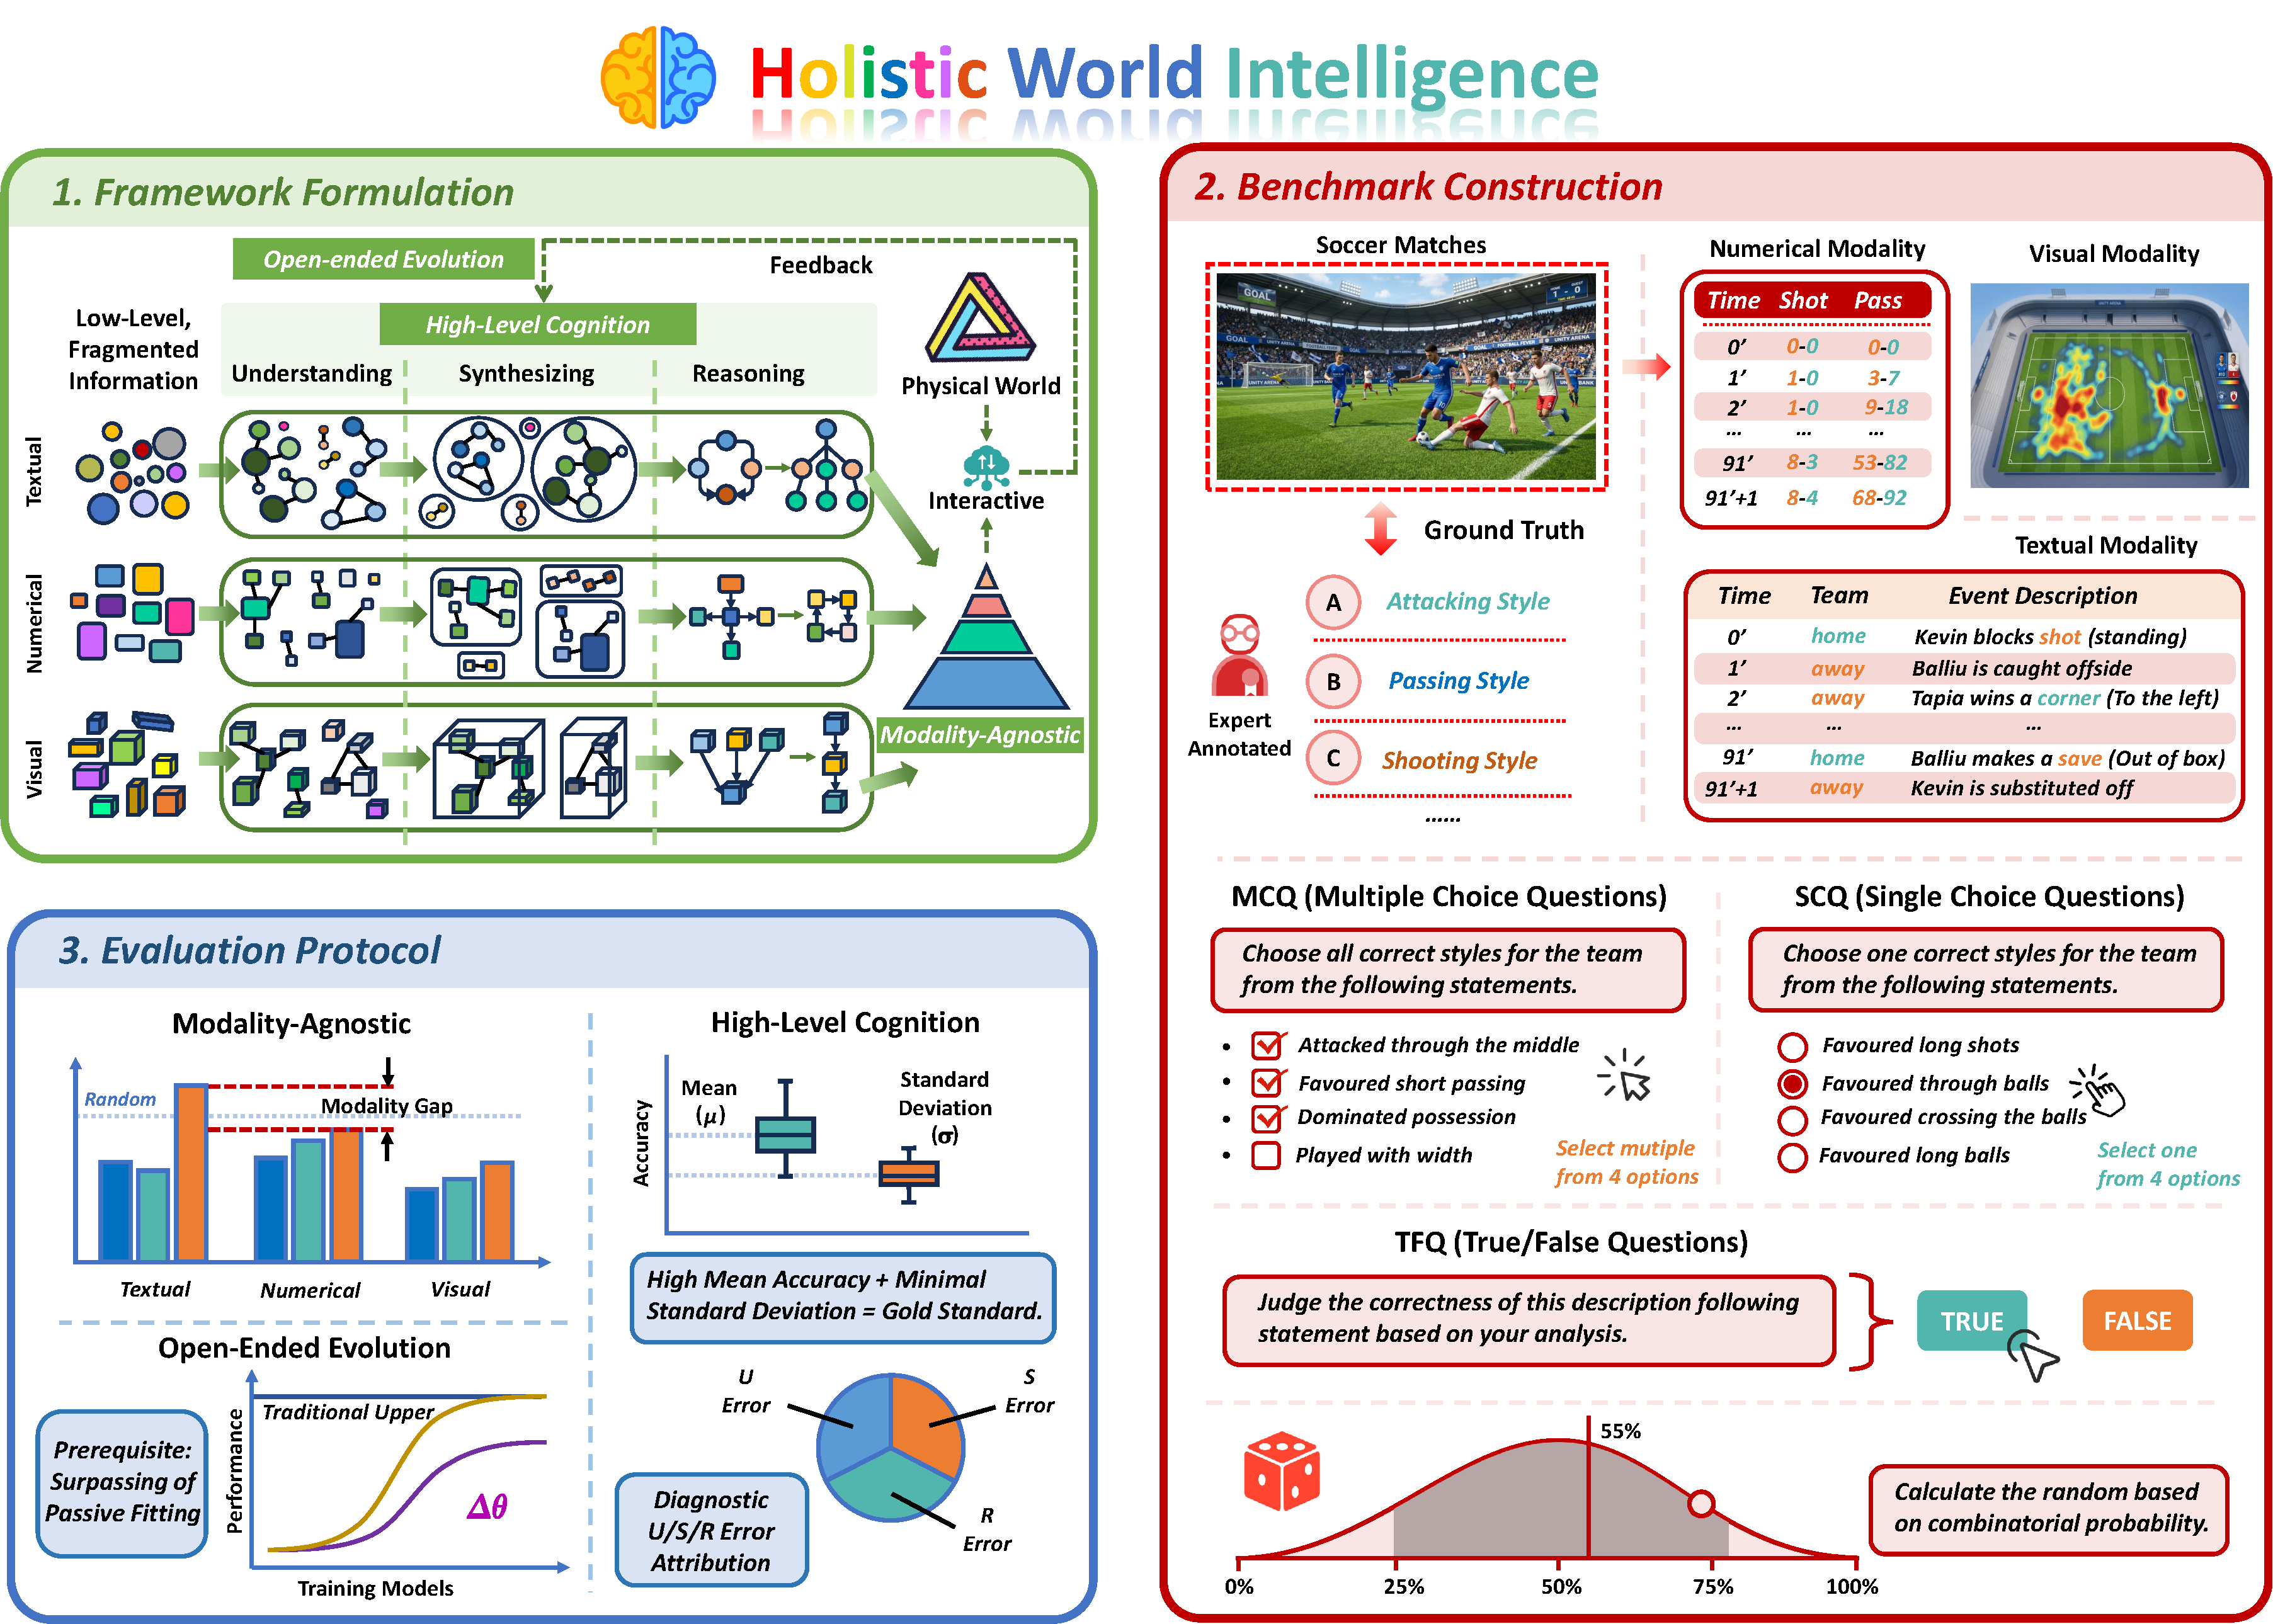
\includegraphics[scale=0.29]{figure/figure2.pdf}
    \vspace{-2mm}
	\caption{The Systematic Paradigm for Evaluating Holistic World Intelligence (HWI) across Multi-modal Representations. }
    \vspace{-3mm}
	\label{figure2}
\end{figure*}

The inherent complexity and heterogeneity of the physical world pose a fundamental bottleneck to the evolution toward Artificial General Intelligence (AGI) \cite{goertzel2014artificial}.
This reality subjects Large Language Models (LLMs)—the quintessential paradigm in the pursuit of AGI \cite{bubeck2023paper}—to foundational performance scrutiny \cite{zhao2023survey}.
Profoundly, addressing this bottleneck necessitates a paradigm shift toward \textbf{Holistic World Intelligence} (HWI), an endogenously and perpetually integrated capacity to process heterogeneous real-world representations.
Inspired by cognitive neuroscience represented by Embodied Multisensory Integration \cite{stein2008multisensory} and Hierarchical Predictive Processing \cite{clark2013whatever}, we posit that HWI can be anchored to three core attributes conceptually illustrated in Figure~\ref{figure1} concretely.
First, HWI is inherently \emph{Modality-Agnostic}, enabling the resolution of heterogeneous physical scenarios through unified internal representations that transcend disparate sensory boundaries \cite{ngiam2011multimodal}.
Second, it embodies \emph{High-Level Cognition} (HLC), mimicking the human-like cognitive hierarchy to integrate foundational functions into structured reasoning chains \cite{laird2017standard, bengio2017consciousness}.
Third, it facilitates \emph{Open-ended Evolution}, a neuroplasticity-inspired attribute \cite{hassabis2017neuroscience} that empowers the model to continuously and actively augment its capabilities through autonomous environmental interaction \cite{silver2021reward}.

Despite their prevalence, current approaches fail to internalize these core attributes of HWI.
Predominantly, while attempting to bridge heterogeneity gaps, Multimodal Large Language Models (MLLMs) largely rely on superficial semantic alignment \cite{radford2021learning} rather than achieving a truly Modality-Agnostic unified representation, leaving them fragmented when facing multidimensional physical properties \cite{wu2024next, tong2024eyes}.
Simultaneously, prevailing reasoning paradigms often focus on scaling exogenous logical complexity via externally designed heuristics \cite{wei2022chain, yao2023tree}; however, such 'plug-and-play' enhancements do not translate into genuine endogenous reasoning capabilities or autonomous cognitive depth \cite{huang2023large}.
Most critically, the current framework still remains restricted to modeling the static physical world through passive data-fitting \cite{kaplan2020scaling}, rather than actively exploring and exploiting dynamic environmental feedback to foster sustained, open-ended cognitive growth \cite{wang2023voyager}.
Consequently, these gaps jointly raise a fundamental question: \emph{Can a unified architecture truly internalize the holistic laws of the physical world to attain authentic, world-level intelligence?}

Fundamentally, overcoming these persistent bottlenecks is currently hindered by systemic deficiencies across three critical dimensions.
Architecturally, the absence of established HWI-centric datasets and evaluation benchmarks \cite{srivastava2022behavior, gu2023maniskill2} precludes a rigorous and empirical measurement of holistic world representations.
Theoretically, a lack of principled analytical guidance consigns the internal mechanisms of world-level cognition to a 'black box' \cite{li2022emergent}, rendering the emergence of HWI largely uninterpretable and opaque \cite{nanda2023progress}.
Methodologically, the dearth of novel paradigms capable of triggering endogenous logical growth and continuous environmental interaction prevents a substantive transition from static fitting to active intelligence augmentation \cite{park2023generative}.
To address these multifaceted gaps, this work establishes a structured framework to rigorously analyze the three defining attributes of HWI, providing both theoretical insights and empirical evidence to guide the development of future effective AGI methodologies \cite{bengio2021deep}.

Therefore, this work establishes a holistic and principled evaluation paradigm to bridge the existing gaps between current LLMs and the realization of authentic AGI \cite{mahowald2024dissociating}. Our specific contributions are summarized across three dimensions:
\begin{itemize}[leftmargin=*]
\item \textbf{Systematic Framework and Infrastructure:} We propose a comprehensive framework for \textbf{Holistic World Intelligence (HWI)}, providing a formal definition of its core attributes (Sec.~\ref{formulation}). To enable empirical measurement, we introduce a specialized benchmark named \emph{WorldScope} (Sec.~\ref{benchmark}) and a rigorous evaluation protocol (Sec.~\ref{protocol}) to assess the emergence of this capability under heterogeneous real-world representations.
\item \textbf{Empirical Investigation of Capability Collapse:} We conduct an extensive empirical study revealing a critical phenomenon we term \textbf{"Capability Collapse"} in current state-of-the-art multimodal models when processing complex physical data (Sec.~\ref{phenomenon}). By delving into the underlying causes of this failure, we provide a foundational analysis that fills the current void in systematic understanding of world-level performance (Sec.~\ref{analysis}).
\item \textbf{In-depth Analysis and Future Roadmap:} We perform a granular investigation into three pillars of HWI: \emph{Modality-Agnosticism} (Sec.~\ref{modality}), \emph{High-level Cognition} (Sec.~\ref{HLC}), and \emph{Open-ended Evolution} (Sec.~\ref{evolution}). Based on these insights, we propose preliminary improvements and offer a strategic roadmap to guide future efforts toward AGI (Sec.~\ref{future}).
\end{itemize}



\begin{table*}[t]
    \centering
    \caption{Comparison of methodologies towards AGI based on the three core attributes of \textbf{Holistic World Intelligence (HWI)}.}
    \vspace{-4mm}
    \label{tab:related_comparison}
    \renewcommand{\arraystretch}{1.0}
    \setlength{\tabcolsep}{4pt} 
    \small 
    \begin{tabularx}{\textwidth}{p{2.8cm} l l X c c c} 
        \toprule
        \textbf{Target Attribute} & \textbf{Major Class} & \textbf{Technical Paradigms} & \textbf{Key Deficiency (vs. HWI)} & \textbf{Mod-A.} & \textbf{HLC} & \textbf{Open-E.} \\
        \midrule
        % 第一组：Modality-Agnostic
        \multirow{2}{*}{\textbf{Modality-Agnostic}} & \multirow{2}{*}{Alignment} 
        & CLIP / Flamingo & Semantically bound to explicit anchors/shortcuts. & \xmark & \xmark & \xmark \\
        & & Knowledge Graphs & Domain-isolated; lacks unified physical grounding. & \xmark & $\triangle$ & \xmark \\
        \midrule
        % 第二组：HLC
        \multirow{2}{*}{\textbf{High-Level Cognition}} & \multirow{2}{*}{Reasoning} 
        & CoT / ToT & Exogenous logic detached from physical constraints. & $\triangle$ & $\triangle$ & \xmark \\
        & & o1 / TTS & Search-based inference without endogenous growth. & $\triangle$ & $\triangle$ & \xmark \\
        \midrule
        % 第三组：Open-E
        \multirow{2}{*}{\textbf{Open-ended Evolution}} & \multirow{2}{*}{Fitting} 
        & Instruction Tuning & Passive interpolation of static, non-interactive data. & $\triangle$ & \xmark & \xmark \\
        & & RLHF / DPO & Reactive optimization lacking proactive world-modeling. & $\triangle$ & $\triangle$ & $\triangle$ \\
        \midrule
        \textbf{All Dimensions} & \textbf{Ours} & \textbf{HWI Framework} & \textbf{Endogenous, grounded, and active intelligence.} & \textbf{\cmark} & \textbf{\cmark} & \textbf{\cmark} \\
        \bottomrule
    \end{tabularx}
    \begin{flushleft}
    \scriptsize
    \textbf{Note}:
    \textbf{Mod-A.}: Modality-Agnostic (transcending sensory boundaries); 
    \textbf{HLC}: High-Level Cognition (endogenously grounded reasoning chains); 
    \textbf{Open-E.}: Open-ended Evolution (active interaction vs. static fitting). 
    \cmark\ indicates strong support; 
    $\triangle$ indicates partial/limited support; 
    \xmark\ indicates little or no support.
    \end{flushleft}
    \vspace{-3mm}
\end{table*}

\begin{table}[t] 
    \centering
    \caption{Summary of existing AGI theoretical perspectives and their gaps relative to the HWI requirements.}
    \vspace{-4mm}
    \label{tab:theory_summary}
    \renewcommand{\arraystretch}{1.0} 
    \setlength{\tabcolsep}{3pt} 
    \footnotesize 
    \begin{tabularx}{\columnwidth}{@{} p{1.3cm} p{2.7cm} X @{}}
        \toprule
        \textbf{Perspective} & \textbf{Core Examples} & \textbf{Primary Gap} \\ 
        \midrule
        \textbf{Optimality} & AIXI, Universal Intelligence & Idealized assumptions; incomputable. \\
        \midrule
        \textbf{Cognitive} & World Models, Active Inference Predictive Processing & Closed environments; modality-specific; limiting unified cross-modal evaluation. \\
        \midrule
        \textbf{Capability} & ARC, Meta-Learning & Static tasks; lacks a unified how-to path. \\
        \midrule
        \textbf{HWI (Ours)} & \textbf{HWI Framework} & \textbf{Integrated, grounded, and evaluable.} \\
        \bottomrule
    \end{tabularx}
    \vspace{-2mm} 
\end{table}

\section{Related Work}
\label{sec:related}

\subsection{Methodological Progress Towards AGI}

Existing AGI methodologies broadly fall into three paradigms (Table~\ref{tab:related_comparison}), each exhibiting systemic deficiencies relative to HWI attributes \cite{marcus2020next}.
First, \textbf{representation alignment} (e.g., contrastive learning, joint embeddings, and models like CLIP \cite{radford2021learning}/Flamingo \cite{alayrac2022flamingo} or Knowledge Graphs \cite{ji2021survey}) maps disparate modalities into shared spaces but remains \emph{semantically bound} to explicit anchors, failing to achieve true \emph{Modality-Agnosticism} \cite{yuksekgonul2022and}.
Second, \textbf{exogenous reasoning} (e.g., CoT, ToT, or search-based paradigms like o1/TTS \cite{snell2024scaling}) facilitates logical transparency yet operates in a "reasoning vacuum" detached from physical constraints, precluding endogenously grounded \emph{High-level Cognition} \cite{pearl2018theoretical}.
Finally, \textbf{static optimization} via instruction tuning or preference learning (RLHF \cite{ouyang2022training}, DPO \cite{rafailov2023direct}) approximates world states through passive data-fitting \cite{bender2020climbing}. Lacking active environmental interaction, these methods cannot sustain \emph{Open-ended Evolution} \cite{lehman2011abandoning}.
The HWI framework is therefore explicitly designed to evaluate and bridge these fundamental gaps between current paradigms and authentic world intelligence \cite{bisk2020experience}.

\vspace{-2mm}
\subsection{Theoretical Progress Towards AGI}

Theoretical studies of AGI have formalized \emph{intelligence} from several distinct but incomplete perspectives (Table~\ref{tab:theory_summary}) \cite{legg2007collection}.
First, \textbf{optimality-based theories} (e.g., AIXI \cite{hutter2005universal}, Universal Intelligence \cite{legg2007universal}) define generality through asymptotic performance across environments \cite{sutton1998reinforcement}.
While principled, they rely on idealized and often incomputable assumptions \cite{leike2017ai}, remaining descriptive rather than executable for real-world interactive intelligence \cite{everitt2018agi}.
Second, \textbf{cognitive and world-model theories} (e.g., World Models \cite{ha2018recurrent}, Predictive Processing \cite{friston2010free}, Active Inference \cite{zhiren2026learning}) emphasize endogenous modeling, prediction, and action \cite{matsuo2022deep}.
Although closer to authentic intelligence, they are typically grounded in specific modalities or closed environments \cite{kaiser2019model}, limiting unified cross-modal evaluation under open-world complexity \cite{hafner2019dream}.
Third, \textbf{capability-oriented theories} (e.g., ARC \cite{chollet2019measure}, meta-learning \cite{finn2017model}) characterize AGI through abstraction, reasoning, and rapid generalization \cite{lake2017building}.
However, they mainly specify \emph{what} capabilities to test, rather than \emph{how} to construct a unified intelligence framework \cite{lecun2022path}, and their largely static tasks are insufficient for continuous interaction and open-ended evolution \cite{team2021open}.
Overall, existing AGI theories clarify important aspects of intelligence, but still lack a unified path from abstract formulation to systematic real-world evaluation \cite{bommasani2021opportunities}.
Our HWI framework addresses this gap through an integrated structure spanning \textbf{framework}, \textbf{benchmark}, and \textbf{protocol}.


\section{Holistic World Intelligence} 
\label{sec:mhlc-benchmark}
\subsection{Framework}
\label{formulation}
Based on the three core attributes of Holistic World Intelligence capabilities in Figure ~\ref{figure2}, we formalize its definition as follows:

1) \textbf{Modality-Agnostic}. Confronted with the complex and heterogeneous representations of the physical world, HWI relies on an underlying, ubiquitous processing mechanism. 
For any given modality $m \in \{\text{num}, \text{vis}, \text{text}, \dots\}$, the macroscopic so-called holistic mechanism of HWI, denoted as $\mathcal{F}$, must satisfy the representational equivalence \cite{baltruvsaitis2018multimodal}. 
Specifically, when disparate modalities $m_a$ and $m_b$ observe the same objective physical event $\mathcal{E}$, this mechanism must transcend representational barriers to ensure absolute consistency in the derived conclusions, fundamentally eliminating reliance on modality-specific or explicit semantic shortcuts:
\begin{equation}
\label{eq1}
\mathcal{F}(\mathcal{X}^{m_a}) \equiv \mathcal{F}(\mathcal{X}^{m_b}) \rightarrow \mathbf{y}_{\mathcal{E}}.
\end{equation}

2) \textbf{High-Level Cognition}. The essence of processing the complex physical world lies in bridging the representational chasm between low-level data and high-dimensional principles. Furthermore, High-Level Cognition can be defined as the transitional process of deriving high-level conclusions from low-level and fragmented foundational information, which can be instantiated as an \emph{Understanding-Synthesizing-Reasoning chain} structure ($f_R \circ f_S \circ f_U$) \cite{liu2025can}. We introduce this paradigm to process heterogeneous physical observations $\mathcal{X}^{m}$: 
\begin{itemize}[leftmargin=*]
    \item \textbf{Understanding-U} ($f_U$): Operates independently on each fragmented, low-level physical segment to extract isolated local features: $\mathcal{H}_{local}^{m} = \{ f_{U}(x_{i}^{m}) \}_{i=1}^{N_{m}}$. 
    \item \textbf{Synthesizing-S} ($f_S$): Integrates all fragmented local features to construct a coherent global representation: $\mathbf{H}_{global}^{m} = f_{S}(\mathcal{H}_{local}^{m})$.
    \item \textbf{Reasoning-R} ($f_R$): Derives high-level conclusions regarding the physical world (e.g., high-dimensional intentions, macroscopic laws) based on this global representation: $\mathbf{y} = f_{R}(\mathbf{H}_{global}^{m})$.
\end{itemize}

3) \textbf{Open-ended Evolution}. Analogous to neuroplasticity in the human brain, the model must achieve continuous reshaping of its endogenous logic through dynamic interaction with the physical environment \cite{parisi2019continual}. This dynamic process exhibits an iterative, upward trajectory alongside the interaction step $t$:
\begin{equation}
\label{eq2}
\theta^{(t+1)} = \theta^{(t)} + \Delta \theta \left( \mathcal{X}_{t}^{m}, \text{Feedback}_{t}, \mathcal{F}_{\theta^{(t)}} \right).
\end{equation}
This ensures the model can continuously shatter its inherent cognitive boundaries and seamlessly adapt to the open-ended, boundless, and complex evolution of the physical world.

\begin{figure}[!t]
	\centering
	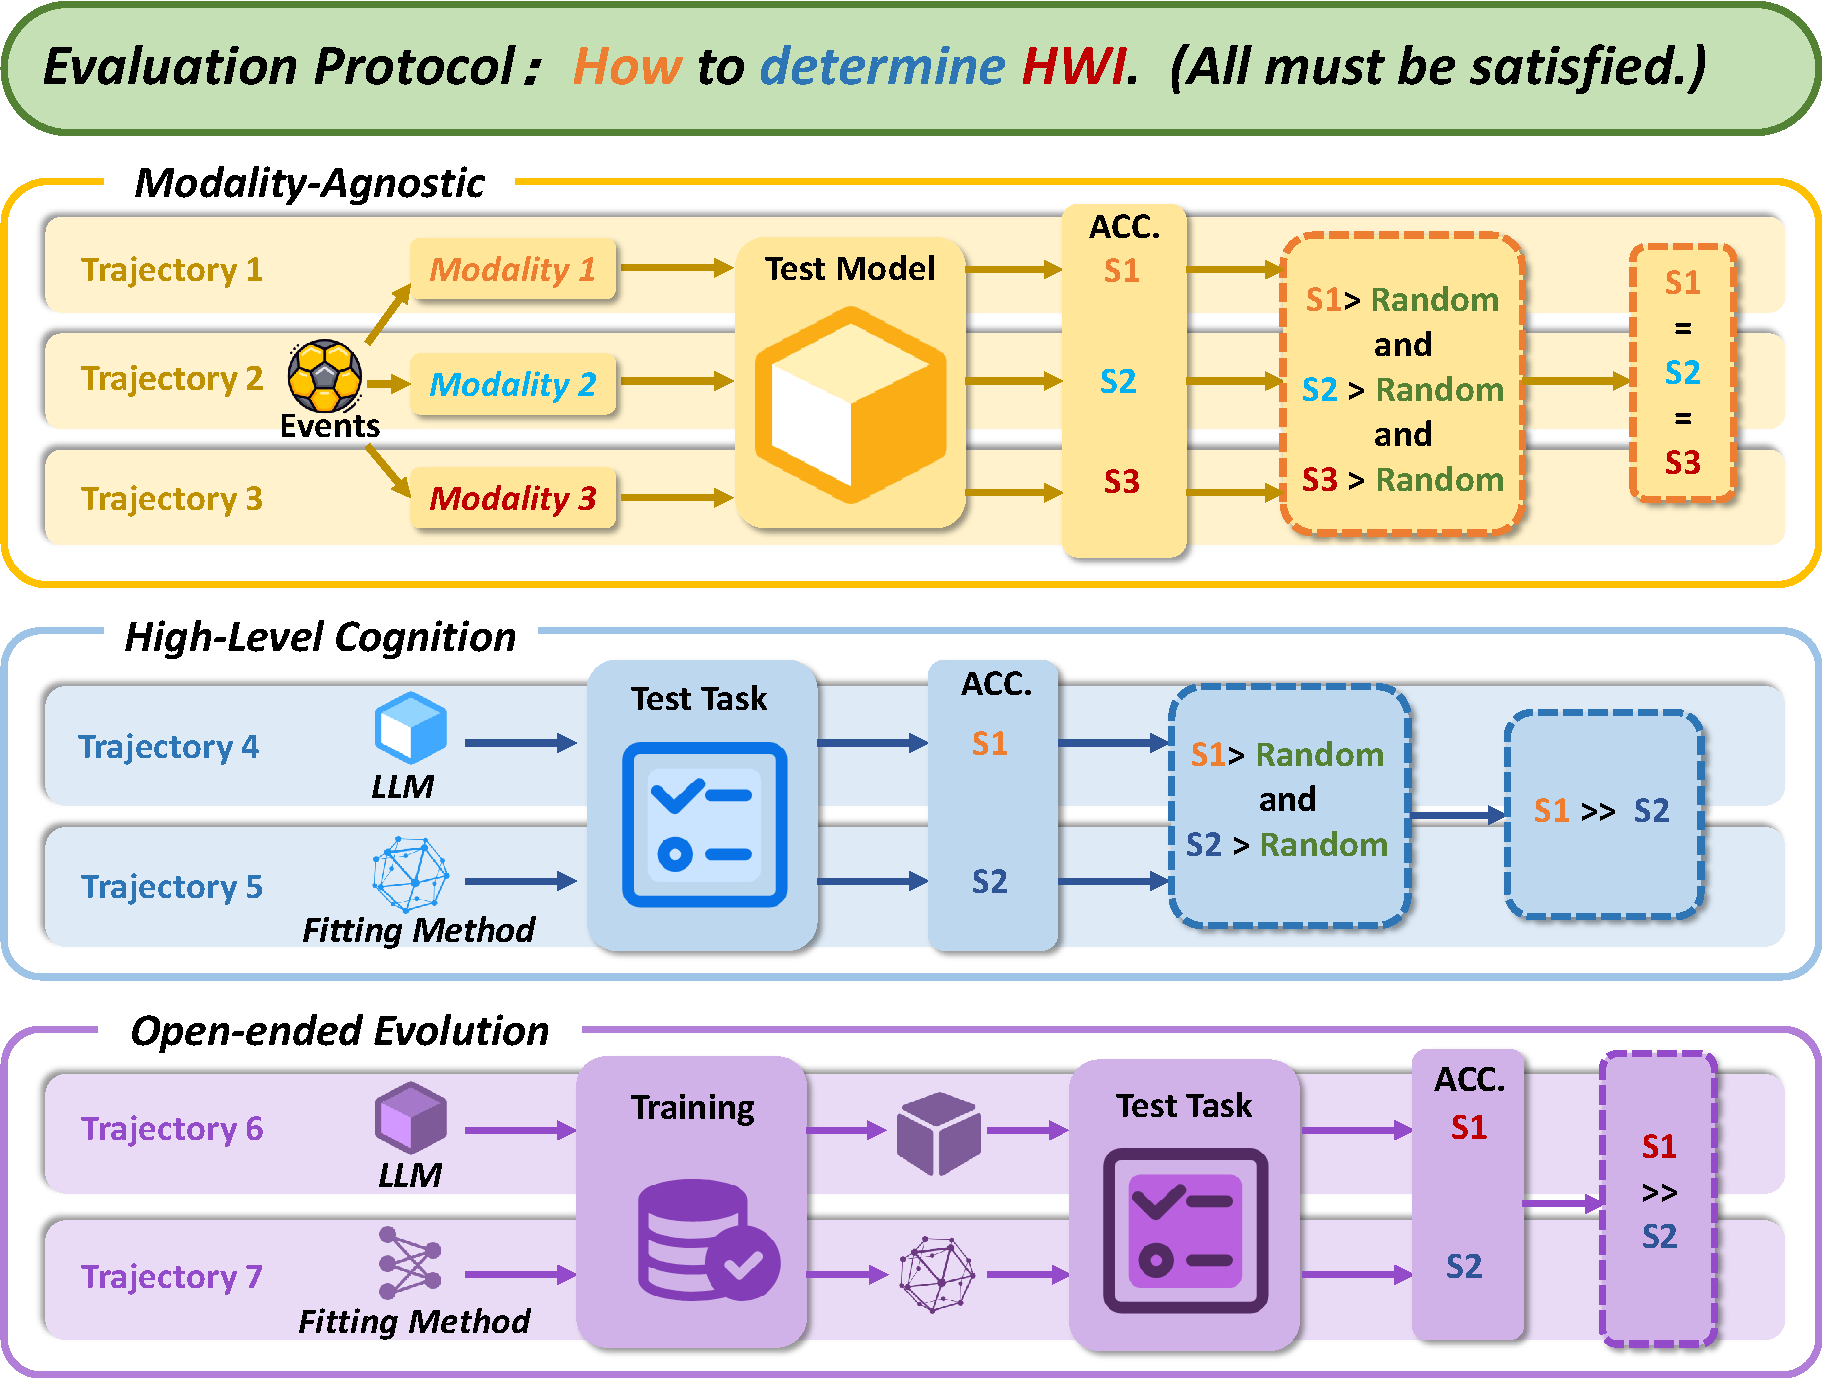
\includegraphics[scale=0.27]{figure/figure10.pdf}
    \vspace{-3mm}
	\caption{Evaluation and Diagnosis pipeline (How to test three capabilities under HWI framework). }
    \vspace{-3mm}
	\label{figure...}
\end{figure}

\subsection{WorldScope Benchmark}
\label{benchmark}

Existing benchmarks predominantly evaluate superficial perception, failing to test models' capacity to \emph{transcend low-level representational barriers} and \emph{formulate high-order macroscopic conclusions}. To address this gap, we introduce \textbf{WorldScope}, a dedicated benchmark for evaluating Holistic World Intelligence, constructing on professional football matches from WhoScored. With the aim at complex physical world characterized by high-dimensional adversarial dynamics, this testbed can rigorously assesses models' HWI capacity boundary. Concretely, WorldScope consists of \emph{two strictly decoupled components} with details in Appendix~\ref{app:construction_pipeline}:
\begin{itemize}[leftmargin=*]
\item \textbf{Low-level Multimodal Input:} We extract fine-grained, fragmented observations for each match, including discrete numerical statistics (e.g., passes, zones), chronological textual commentary, and visual positional heatmaps of all players, while depicting the underlying physical world.
\item \textbf{High-level Integrated Output:} Macroscopic team-style summaries are extracted from various Expert Match Reports and normalized into a finite set of 12 tactical playing styles, which cannot be trivially deduced from isolated foundational data.
\end{itemize}

These strictly decoupled components then perfectly operationalizes our theoretical framework. 
(1) First, by capturing the exact same objective physical event across three heterogeneous channels, the benchmark inherently demands \textbf{Modality-Agnostic} processing, preventing models from exploiting modality-specific semantic shortcuts. 
(2) Furthermore, bridging the representational chasm between raw, fragmented signals and macroscopic tactical labels necessitates genuine \textbf{High-Level Cognition}. Specifically, a model must first perform \textit{understanding} by extracting isolated local features from fragmented inputs (e.g., recognizing discrete passes or shots event from numerical counts, textual commentary, or visual density spots). Next, it must execute \textit{synthesizing} by integrating these scattered events into a coherent global representation (e.g., a panoramic view of the overall match dynamics). Finally, through \textit{reasoning}, it maps this unified representation to high-level conclusions (e.g., deducing macroscopic tactical styles like "favoured short passing"). This process comprehensively forces the model to execute a complete "Understanding-Synthesizing-Reasoning" (U/S/R) cognitive chain. 
(3) Crucially, our continuous real-world football seasons inherently supports \textbf{Open-ended Evolution}. This provides an infinitely renewable environment, allowing models to not only be statically evaluated but also continuously trained to adapt to novel tactical trends, thereby iteratively evolving their alignment with real-world dynamics. 

% Because new matches and expert reports are generated perpetually, the dataset seamlessly scales without the bottleneck of expensive human annotation.
% We curated a substantial dataset of 5,000 matches to ensure robust evaluation. 

As for benchmark's diversity and richness, to mitigate the ambiguity of HWI evaluation, we formulate the testbed into standardized objective tasks: Multiple Choice Questions (MCQ), Single Choice Questions (SCQ), and True/False Questions (TFQ). For consistency, instruction semantics are strictly aligned across all modalities. We also adopt Exact-Match (EM) as accuracy metric after filtering, where any generated content falling outside the finite acceptable ground truth set is categorically penalized as an incorrect response during HWI evaluation.


\begin{table*}[t]
    \centering
    \caption{Comprehensive performance comparison on three modalities (textual, numerical, and visual) and three tasks (MCQ, SCQ, and TFQ). $\dagger$ denotes theoretically calculated values. }
    \vspace{-2mm}
    \label{tab:main_results_hierarchical}
    \renewcommand{\arraystretch}{1.0} 
    \setlength{\tabcolsep}{14pt} % 
    \begin{tabular}{@{} l l c c c c @{}}
        \toprule
        \multirow{2}{*}{\textbf{Category}} & \multirow{2}{*}{\textbf{Model}} & \multirow{2}{*}{\textbf{Params}} & \multicolumn{3}{c}{\textbf{Accuracy (\%)}} \\
        \cmidrule(lr){4-6} 
        & & & \textbf{MCQ} & \textbf{SCQ} & \textbf{TFQ} \\
        \midrule
        
        % ==========================================
        % 基线部分
        % ==========================================
        Baseline & Random-Level & - & 12.95$^\dagger$ & 30.81$^\dagger$ & 56.74$^\dagger$ \\
        \midrule
        
        % ==========================================
        % 文本模态
        % ==========================================
        \rowcolor{blue!10} \multicolumn{6}{c}{\textit{Textual Modality}} \\
        \midrule

        \multirow{6}{*}{General (Zero-Shot)} 
         &  GPT-5.4 \cite{singh2025openai} & - & $\underline{15.00} \pm 3.16$ & $\underline{36.20} \pm 4.87$ & $\underline{54.23} \pm 5.11$ \\
        & Claude-4.6-opus \cite{mukherjee2026red} & - & $14.40 \pm 2.06$ & $33.20 \pm 4.53$ & $53.54 \pm 2.28$ \\
        & Llama-3.1 \cite{grattafiori2024llama} & ~70B & $11.60 \pm 3.26$ & $35.60 \pm 6.62$ & $53.47 \pm 6.30$  \\
        & Mistral-Small-3 \cite{liu2026ministral} & ~24B & $9.00 \pm 4.20$ & $33.60 \pm 5.95$ & $50.89 \pm 3.81$ \\
        & Qwen-2.5 \cite{yang2025qwen3} & ~3B & $\textcolor{blue}{7.20} \pm 2.71$ & $20.80 \pm 5.11$ & $\textcolor{blue}{38.13} \pm 6.72$ \\
        & vicuna-1.5 \cite{zheng2023judging} & ~7B & $8.40 \pm 1.36$ & $\textcolor{blue}{14.60} \pm 1.62$ & $50.00 \pm 0.00$ \\
        \cmidrule(l){2-6} 
        
        \multirow{3}{*}{Traditional Architecture} 
        & \textbf{LSTM} \cite{hochreiter1997long} & ~4.60M &  $20.00 \pm 3.85$ & $\mathbf{\textcolor{red!60!black}{37.20}} \pm 4.07$ & $\mathbf{\textcolor{red!60!black}{61.74}} \pm 2.27$ \\
        & \textbf{MLP} \cite{rumelhart1986learning} & ~3.98M & $17.20 \pm 1.47$ & $ 33.60 \pm 2.24$ & $58.28 \pm 2.77$ \\
        & \textbf{GRU} \cite{cho2014learning} & ~4.44M & $\mathbf{\textcolor{red!60!black}{21.00}} \pm 2.28$ & $ 36.60 \pm 3.79$ & $60.05 \pm 2.26$ \\
        \midrule

        % ==========================================
        % 数字模态
        % ==========================================
        \rowcolor{orange!10} \multicolumn{6}{c}{\textit{Numerical Modality}} \\
        \midrule
        
        \multirow{6}{*}{General (Zero-Shot)} 
        &  GPT-5.4 \cite{singh2025openai} & - & $10.40 \pm 2.94$ & $33.40 \pm 6.89$ & $54.22 \pm 6.22$ \\
        & Claude-4.6-opus \cite{mukherjee2026red} & - & $\underline{14.40} \pm 3.61$ & $\underline{36.40} \pm 8.27$ & $\underline{56.36} \pm 8.92$  \\
        & Llama-3.1 \cite{grattafiori2024llama} & ~70B & $6.40 \pm 2.42$ & $25.40 \pm 5.54$ & $54.21 \pm 8.67$ \\
        & Mistral-Small-3 \cite{liu2026ministral} & ~24B & $\textcolor{blue}{5.80} \pm 2.64$ & $22.40 \pm 4.88$ & $53.03 \pm 4.53$ \\
        & Qwen-2.5 \cite{yang2025qwen3} & ~3B & $6.00 \pm 0.63$ & $24.80 \pm 3.37$ & $\textcolor{blue}{36.84} \pm 5.95$ \\
        & vicuna-1.5 \cite{zheng2023judging} & ~7B & $12.40 \pm 1.74$ & $\textcolor{blue}{13.80} \pm 0.98$ & $50.00 \pm 0.00$ \\
        \cmidrule(l){2-6} 
        
        \multirow{3}{*}{Traditional Architecture} 
        & \textbf{CNN} \cite{lecun1989backpropagation} & ~0.40M & $23.80 \pm 3.31$ & $ 36.80 \pm 4.71$ & $63.38 \pm 5.65$ \\
        & \textbf{MLP} \cite{rumelhart1986learning} & ~0.43M & $\mathbf{\textcolor{red!60!black}{28.40}} \pm 4.22$ & $\mathbf{\textcolor{red!60!black}{38.80}} \pm 6.68$ & $\mathbf{\textcolor{red!60!black}{63.87}} \pm 4.37$ \\
        & \textbf{GRU} \cite{cho2014learning} & ~0.25M & $24.00 \pm 4.82$ & $32.40 \pm 5.78$ & $60.48 \pm 3.48$ \\
        \midrule
        
        % ==========================================
        % 图像模态
        % ==========================================
        \rowcolor{green!10} \multicolumn{6}{c}{\textit{Visual Modality}} \\
        \midrule
        
        \multirow{6}{*}{General (Zero-Shot)} 
        &  GPT-5.4 \cite{singh2025openai} & - & $8.60 \pm 0.49$ & $26.80 \pm 2.56$ & $52.02 \pm 2.39$ \\
        & Claude-4.6-opus \cite{mukherjee2026red} & - & $11.40 \pm 1.36$ & $\underline{30.60} \pm 5.00$ & $\underline{56.59} \pm 3.55$ \\
        &  Llama-3.2-Vision \cite{grattafiori2024llama} & ~90B &  $7.60 \pm 1.36$ & $21.00 \pm 2.28$ & $\textcolor{blue}{32.55} \pm 4.28$  \\
        & Mistral-Small-3.1 \cite{liu2026ministral} & ~24B & $9.00 \pm 3.63$ & $30.20 \pm 4.26$ & $55.00 \pm 1.89$ \\
        & Qwen-2.5-VL \cite{bai2025qwen3} & ~3B & $\underline{12.00} \pm 2.19$ & $14.80 \pm 3.76$ & $49.26 \pm 5.52$ \\
        & LLaVa-1.5 \cite{liu2024improved} & ~7B & $\textcolor{blue}{5.40} \pm 0.49$ & $\textcolor{blue}{13.40} \pm 2.58$ & $50.00 \pm 0.00$  \\
        \cmidrule(l){2-6}
        
        \multirow{3}{*}{Traditional Architecture} 
        & \textbf{ResNet-18} \cite{he2016deep} & ~11.31M & $21.40 \pm 2.58$ & $35.00 \pm 5.40$ & $62.26 \pm 5.33$ \\
        & \textbf{DenseNet-121} \cite{huang2017densely} & ~7.22M & $23.20 \pm 2.79$ & $35.20 \pm 4.71$ & $60.47 \pm 2.26$ \\
        & \textbf{EfficientNet-B0} \cite{tan2019efficientnet} & ~4.34M & $\mathbf{\textcolor{red!60!black}{24.40}} \pm 2.94$ & $\mathbf{\textcolor{red!60!black}{37.60}} \pm 4.72$ & $\mathbf{\textcolor{red!60!black}{63.11}} \pm 1.85$ \\
        
        \bottomrule
    \end{tabular}
    \vspace{-2mm}
\end{table*}



\subsection{Evaluation Protocol}
\label{protocol}

To systematically bridge the empirical results through WorldScope Benchmark with the theoretical foundations under HWI framework, we establish a rigorous evaluation protocol to shift the theoretical perspective to a verifiable sanity check. In this view, the protocol is specifically designed to diagnose quantitatively whether the tested model sufficiently exhibits three formalized attributes of HWI.

1) \textbf{Modality-Agnostic Check:} \emph{Cross-Modality Alignment.} 
To empirically validate the representational equivalence ~\ref{eq1}, we evaluate models independently across numerical ($m_{num}$), textual ($m_{text}$), and visual ($m_{vis}$) modalities for the same split of objective physical events $E$. 
% A model possessing true HWI should yield highly consistent predictive results regardless of the input modality. 
By juxtaposing the performance across heterogeneous input channels, we can measure this "modality gap". 
% Crucially, this evaluation must be strictly anchored against a mathematical random baseline. 
% Comparing against random chance is theoretically imperative to establish foundational validity; mere consistency across modalities is mathematically meaningless if the model is systematically hallucinating or guessing. 
% However, exceeding the random baseline is merely a necessary prerequisite, not a sufficient condition. 
To truly prove models' holistic mechanism $\mathcal{F}$ transcending representational barriers, a model must simultaneously satisfy two rigorous criteria: (1) it must significantly exceed the \emph{random baseline} across all modalities, and (2) it must exhibit a \emph{minimized modality gap}.
% Macro-statistical convergence is deceptive if a model correctly predicts disjoint subsets of samples across different modalities. 
In this case, genuine Modality-Agnosticism mandates that for any specific physical event $E_i \in E$, the derived macroscopic truth $y_i$ must remain invariant across $m_{num}$, $m_{text}$, and $m_{vis}$. 
Then, by sanity check on degradation among modalities, a persistent reliance on modality-specific semantic shortcuts is exposed, thereby invalidating any claim of modality-agnostic capability.


2) \textbf{High-Level Cognition Check:} \emph{Statistical Aggregation and Diagnostic Attribution for $f_R \circ f_S \circ f_U$.} 
To quantify a model's capacity to execute the "Understanding-Synthesizing-Reasoning" chain, we introduce a mean-and-standard-deviation ($\mu \pm \sigma$) profiling strategy. 
First, we need to check \emph{whether models are capable of HLC capability}.
In this case, we have mean accuracy $\mu$ serving as the primary indicator of model's absolute capacity to successfully complete the full mapping from fragmented inputs to high-order conclusions as $y = f_R(f_S(f_U(x)))$, while the standard deviation $\sigma$ quantifies the internal stability of this cognitive chain against data variance. 
Here, models are required to surpass the boundary achieved by task-specific traditional-architecture models with passive data-fitting to empirically establish the genuine, intrinsic emergence of HLC.
Futhermore, we need to check \emph{whether models have the intrinsic ability of HLC capability}.
% Because these compact architectures establish a physical upper bound for "passive data-fitting" within a closed data distribution, a massive foundation model that fails to outperform them in a zero-shot setting fundamentally demonstrates an inability to autonomously construct a genuine endogenous reasoning chain.
% If a model's pre-trained, generalized cognitive capacity is inferior to simple statistical interpolation, any claim of possessing High-Level Cognition is entirely invalidated.  
To pinpoint exact structural bottlenecks when this cognition fails, we introduce a diagnostic U/S/R error attribution mechanism in Appendix ~\ref{sec:usrules}). 
This allows us to deconstruct incorrect predictions and identify precisely which specific sub-function—local feature extraction $f_U$, global integration $f_S$, or high-dimensional deduction $f_R$—fractures when processing complex physical signals.

3) \textbf{Open-ended Evolution Check:} \emph{Evolutionary Baselines vs. Superficial Fitting.} 
Our formulation \ref{eq2} mandates that an intelligent agent can autonomously and structurally reshape its internal logic through environmental interaction. 
To investigate this potential, we benchmark general LLMs against two distinct reference points: traditional task-specific supervised models and fully fine-tuned LLMs. 
Here, traditional-architecture models establish a physical upper bound for "passive data-fitting". 
By further evaluating LLMs before and after task-specific fine-tuning, we can diagnose the nature of their learning and evolution capabilities. 
If the fine-tuned LLMs still fail to surpass the traditional-architecture baselines, it constitutes powerful \emph{counter-evidence} indicating that the parameter updates merely resulted in superficial overfitting to task distribution, rather than triggering the genuine, endogenous structural cognitive growth required for true open-ended evolution.


\vspace{-2mm}

\section{Experiment}
\label{sec:experiment}
\subsection{Experimental Setup}
\textbf{Dataset Configurations}. The experiments are performed on WorldScope benchmark comprising 5,000 examples in total, with 4,500 examples for training and 500 for testing. All models will be tested on the same test split with \emph{three assessment forms} (SCQ, MCQ, and TFQ), and instantiated via prompt templates for \emph{three modality inputs} (textual, numerical, and visual).

\textbf{Comparison Models}. To provide sufficient experimental evidence for subsequent argumentation under protocal in ~\ref{protocol}, we will test with SOTA LLMs of various modalities on the same backbone families before and after fine-tuning, while taking traditional architecture models as the capability boundary of passive data-fitting method. The full experiment details including model list, input formatting, training, and hyperparameters) are given in Appendix ~\ref{sec:training-protocol}.


\subsection{Main Result and Analysis}
\label{phenomenon}

Table ~\ref{tab:main_results_hierarchical} presents a comprehensive performance comparison across textual, numerical, and visual modalities, encompassing general-purpose LLMs alongside the capability boundary of the passive data-fitting method presented by task-specific traditional-architecture models. The empirical data intuitively reveals several highly counter-intuitive phenomena exhibited by these SOTA LLMs confronting complex physical world representations.

1) \textbf{The Inverse Scaling Phenomenon.}
Contemporary AI development relies heavily on \emph{Scaling Laws}, which posit that model capabilities scale monotonically with parameter count. 
However, our experimental results reveal a counter-intuitive "inverse scaling" phenomenon. 
In the numerical modality, Llama-3.1 (70B) and Mistral-Small-3 (24B) yield MCQ accuracies of 6.40\% and 5.80\%, respectively. 
Not only are these performances inferior to the significantly smaller Vicuna-1.5-7B (MCQ: 12.40\%), but they are also comprehensively dominated by a simple CNN architecture with a mere 0.40M parameters (MCQ: 23.80\%) by a margin of over three times. 
Similarly, in the visual modality, the 90B-parameter Llama-3.2-Vision falls far behind the 4.34M-parameter EfficientNet-B0. 
This stark contrast—where million-parameter networks absolutely suppress hundred-billion-parameter LLMs—intuitively demonstrates that when confronting specific structural regularities of the physical world, merely \emph{scaling up parameters} results in computational redundancy rather than the emergence of \emph{genuine problem-solving capabilities}.

2) \textbf{Hallucination and Fragility of LLMs.}
The Mean and Standard Deviation reported in the table reflects not only the absolute performance but also directly exposes the \emph{stability and epistemic certainty} of the model outputs.
It can be observed that general LLMs are pervasively accompanied by exceptionally high standard deviations across various physical tasks. 
For instance, Llama-3.1 70B scores 54.21\% ± 8.67\% on the numerical TFQ task, and Claude-4.6-opus even reaches 56.36\% ± 8.92\%. 
In contrast, lightweight models (e.g., ResNet-18, EfficientNet-B0) consistently exhibit not only higher means but also significantly lower variances (e.g., EfficientNet-B0 achieving 63.11\% ± 1.85\% on visual TFQ).
Such \emph{drastic performance fluctuations}with standard deviations reaching 8-9 percentage points directly expose the extreme \emph{Logical Fragility} underlying these LLMs. 
In this case, their representational outputs are highly susceptible to random noise in the input context or minor perturbations in the prompt, essentially degenerating into severe hallucination and random guessing. 
% This proves that architectures equipped with appropriate inductive biases can formulate robust and deterministic reasoning logic when addressing physical tasks.

\begin{figure}[!t]
	\centering
	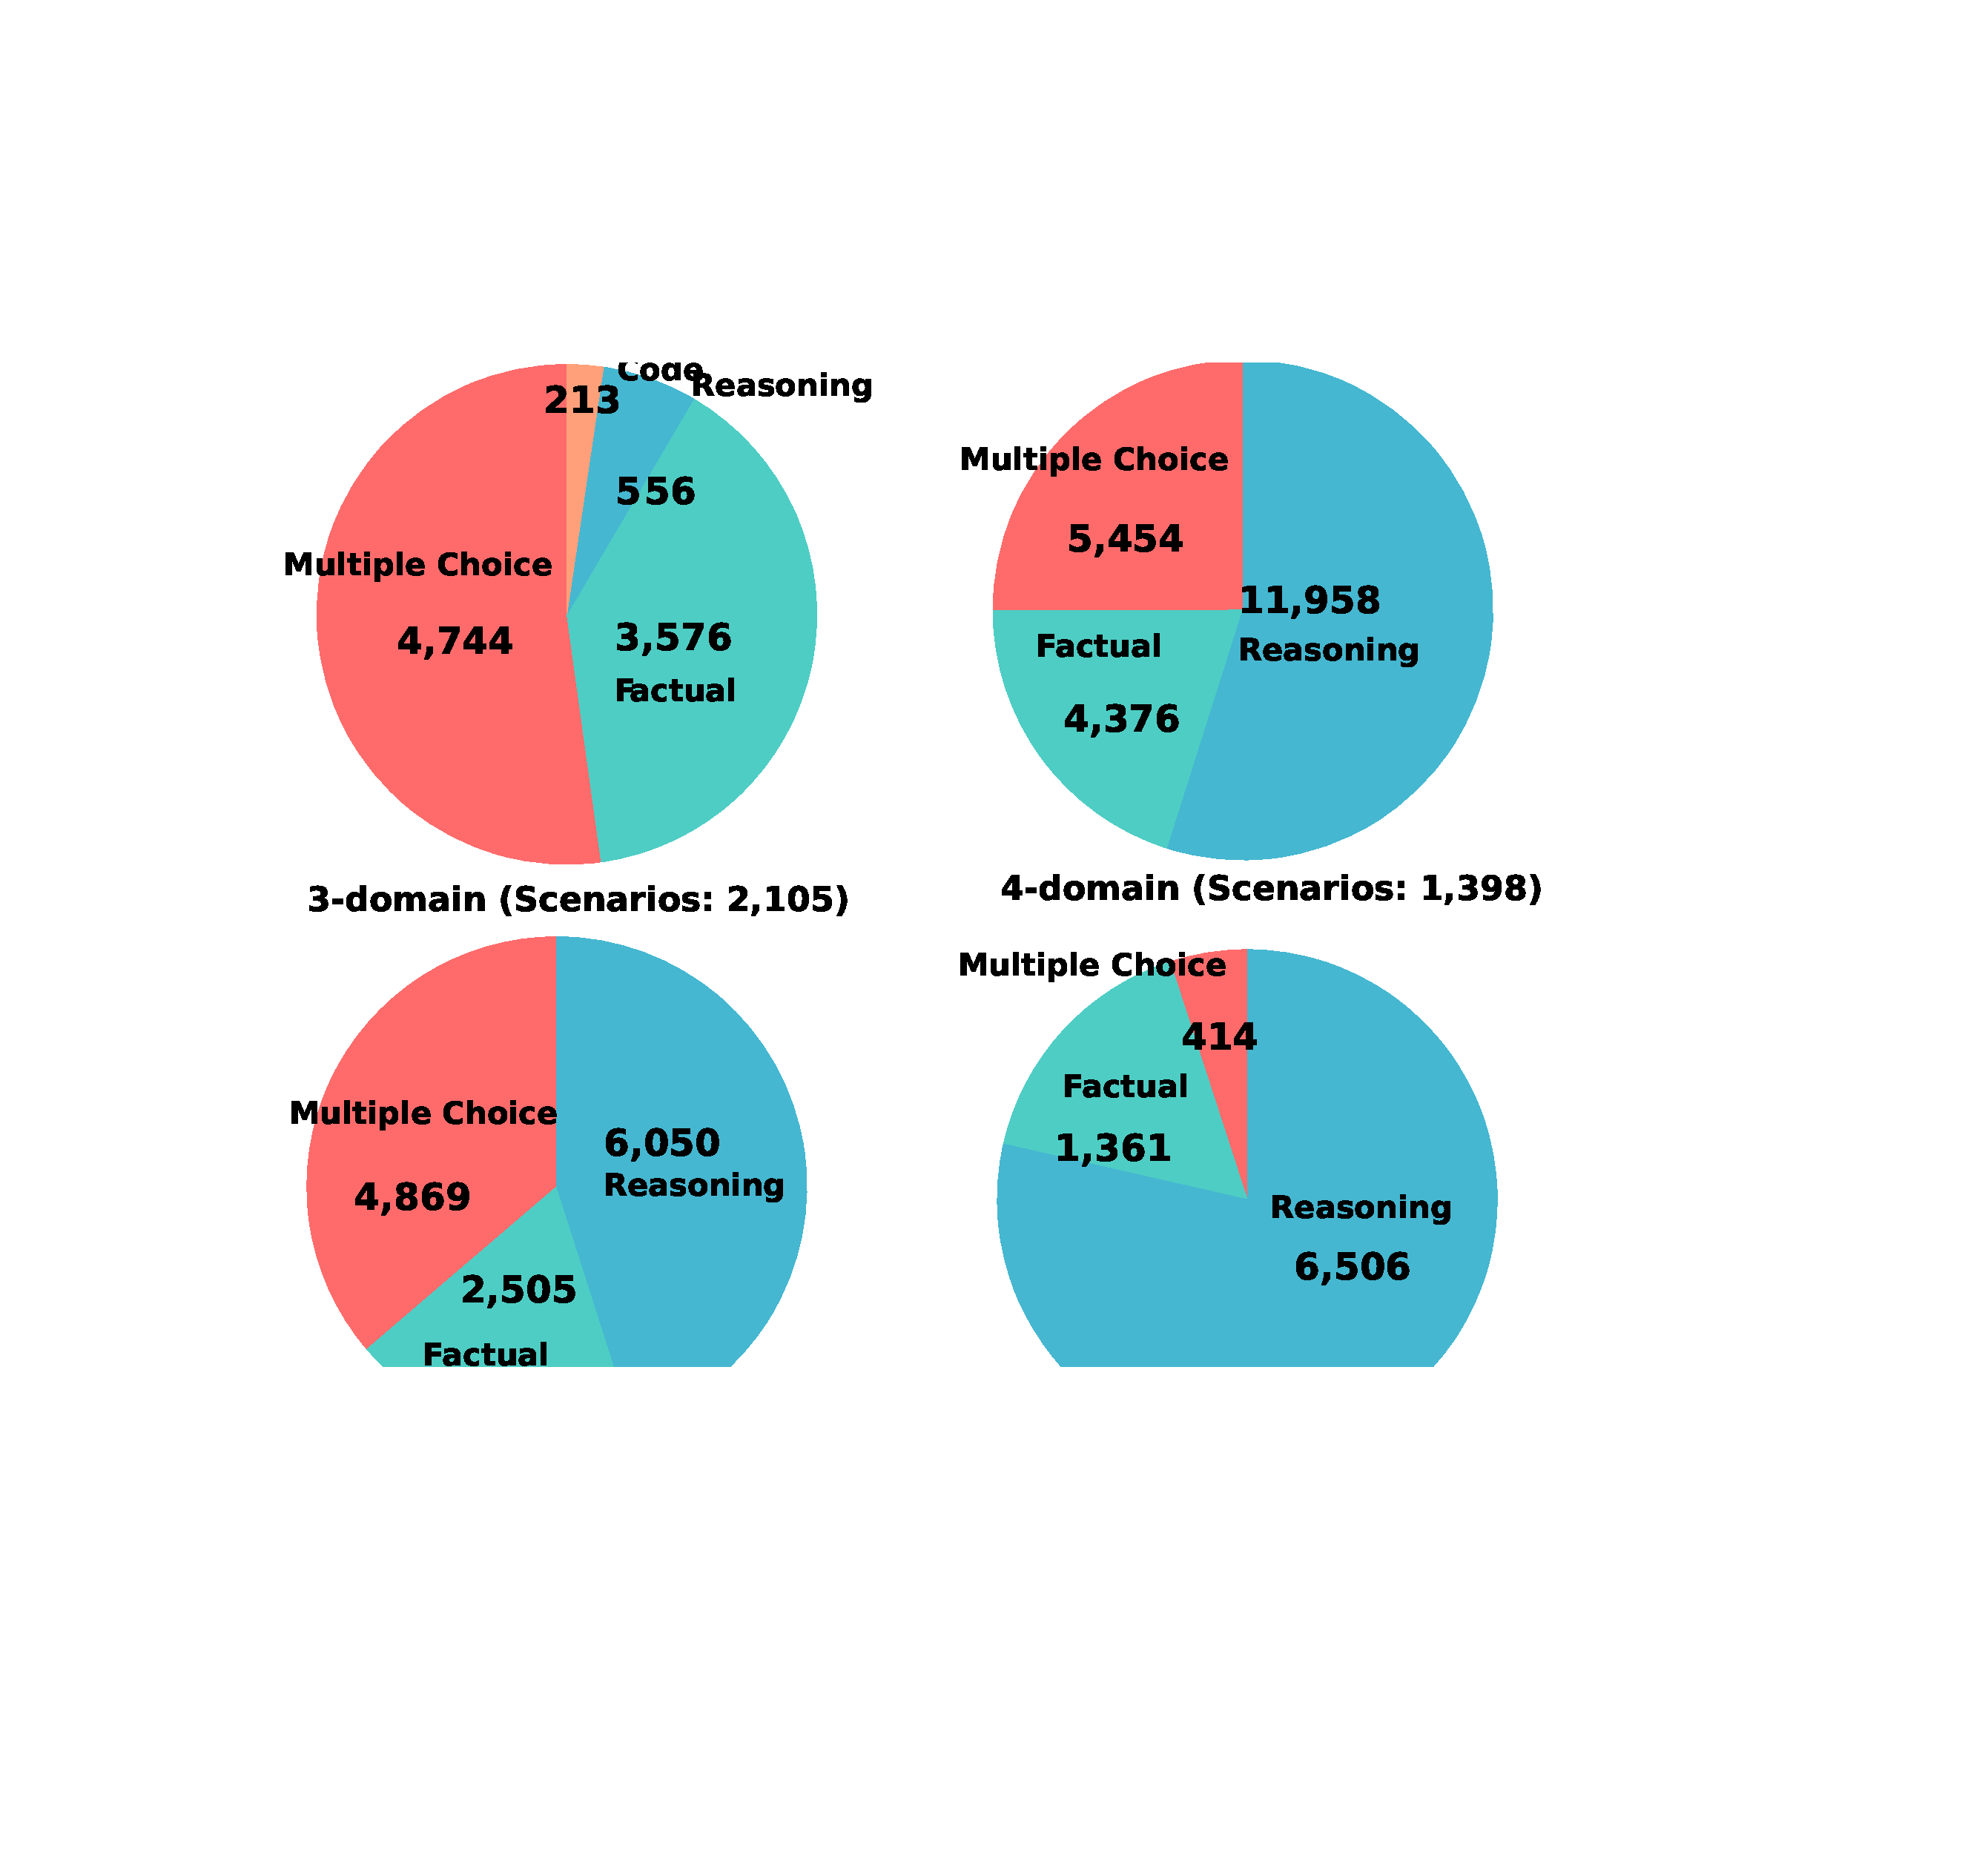
\includegraphics[width=\linewidth]{figure/position.pdf}
    \vspace{-5mm}
	\caption{Modality-Agnostic properties along with different models and different problem tasks}
	\label{fig:cross-modality}
    \vspace{-5mm}
\end{figure}

\subsection{Insight of Capability Collapse}
\label{analysis}
1) \textbf{Complete performance crash.} 
It is widely accepted that the models we tested have represented the capability upper bound of current LLMs.
By contrast, GPT-5.4 scores a mere 8.60\% on MCQ, 26.80\% on SCQ, and 52.02\% on TFQ in the visual modality—falling strictly below the pure random guessing threshold across all three metrics.
Claude-4.6-opus exhibits a similarly dismal and comprehensive collapse (MCQ: 11.40\%, SCQ: 30.60\%, TFQ: 56.59\%).
Therefore, this perceived "ceiling" is now facing a \emph{catastrophic failure} under our evaluation framework across all task formats.
These empirical evidences reveal that these apex models would even fail to reach the mathematical upper probability of random chance, regardless of problem tasks.

2) \textbf{Incompatibility between architecture and physical world.}
More crucially, even within their native and most proficient textual modality, the performance of these top-tier models still remains fundamentally constrained. 
While GPT-5.4 and Claude-4.6-opus barely manage to cross the random baseline on textual MCQ and SCQ, they persistently fall below the baseline on TFQ (e.g., GPT-5.4: 54.23\%, Claude-4.6-opus: 53.54\%). 
Furthermore, they are comprehensively outperformed by the traditional lightweight LSTM architecture across the entire metric matrix (MCQ: 20.00\%, SCQ: 37.20\%, TFQ: 61.74\%).
This persistent cross-modal degradation intuitively proves that the capability collapse of LLMs on heterogeneous physical world tasks is not an accidental byproduct of format complexity or insufficient training.
On the contrary, it exposes that the entire \emph{autoregressive next-token prediction paradigm} itself inherently possesses an \emph{insurmountable capability ceiling}.



\begin{figure}[!t]
	\centering
	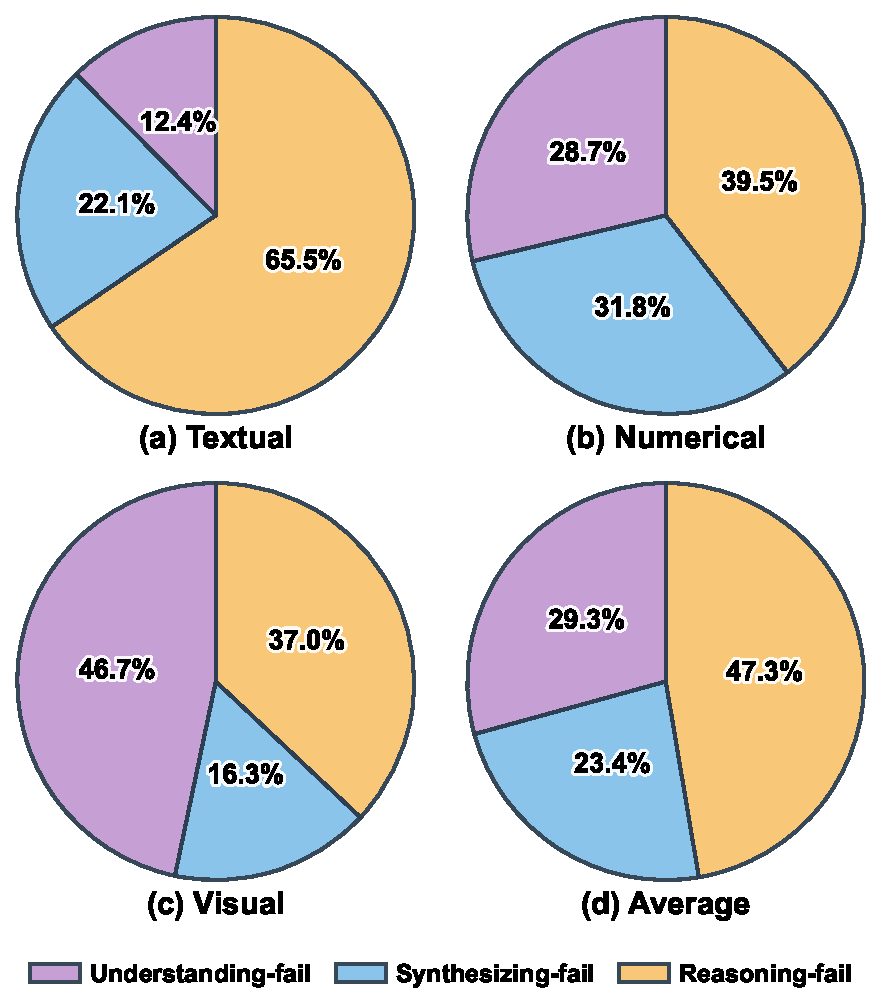
\includegraphics[width=0.90\linewidth]{figure/figure15.pdf}
	\caption{Error Attribution across the U/S/R Chain, exposing the fragility of High-Level Cognition in LLMs.}
	\label{fig:HCL}
\end{figure}

\section{Discussion}
\label{sec:discussion}

This section fundamentally and insightfully explores the underlying mechanisms of this collapse and its implications for future real Artificial General Intelligence (AGI). 

Specifically, we deconstruct the collapse into deficits across \textbf{three core characteristics}: 
(i) the \emph{violation of Modality-Agnosticism}, evaluated via cross-modal performance comparisons; 
(ii) the \emph{breakdown of High-Level Cognition}, analyzed through error attribution along the Understanding-Synthesizing-Reasoning (U/S/R) chain; 
and (iii) the \emph{absence of Open-ended Evolution}, demonstrated by contrasting general LMs, fine-tuned LMs, and traditional architectures. 
% Furthermore, we stress-test the models using few-shot learning to rule out shallow causes like insufficient context. 
Finally, we highlight the \textbf{evolutionary bottlenecks} in the current AGI trajectory and outline future directions.

\begin{figure}[!t]
	\centering
	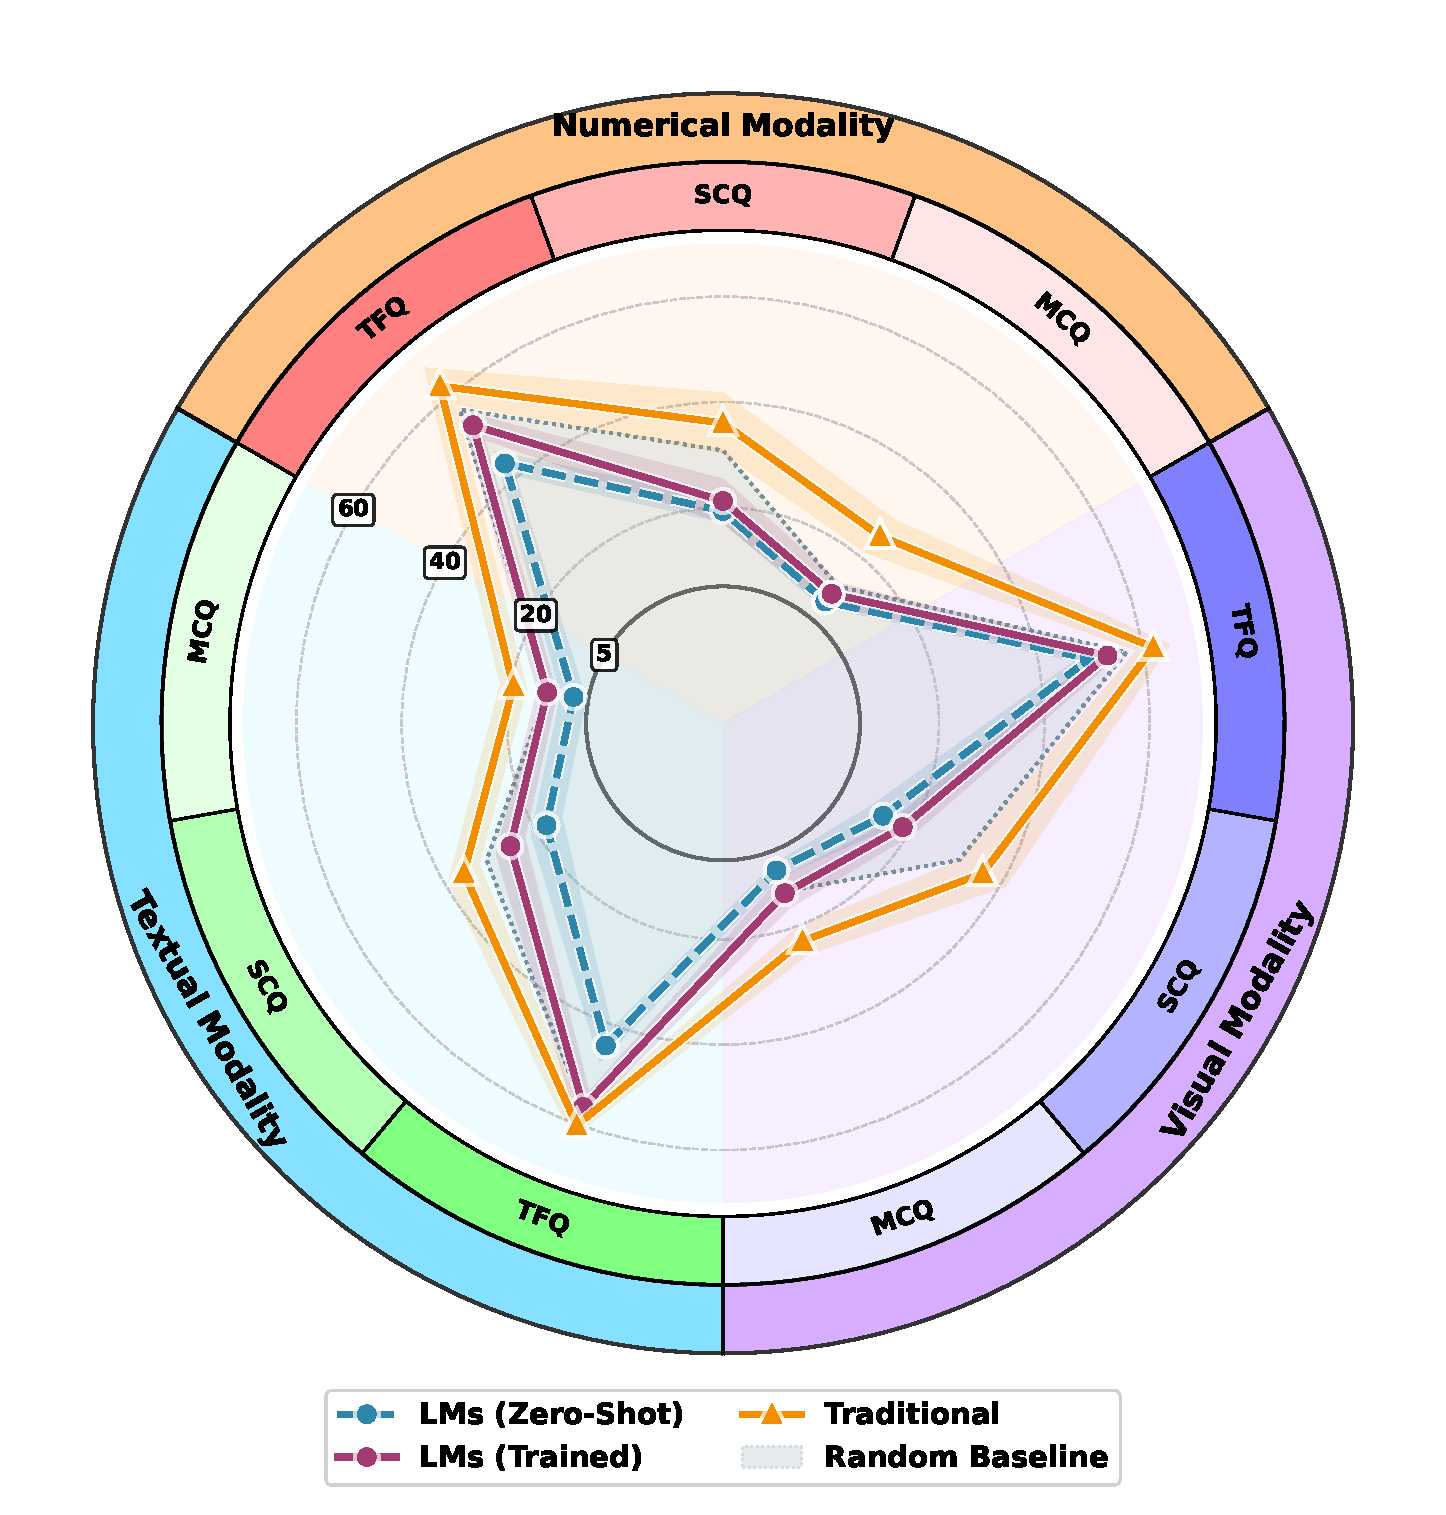
\includegraphics[width=\linewidth]{figure/figure7.pdf}
	\vspace{-5mm}
    \caption{Evaluation of Open-Ended Evolution comparing LLMs and traditional-architecture models across modalities.}
    \vspace{-4mm}
	\label{fig:evolution}
\end{figure}

\subsection{Modality-Agnosticism}
\label{modality}

To evaluate the \textit{Modality-Agnostic} capability, we analyze performance across different modalities with various problem tasks illustrated in Figure ~\ref{fig:cross-modality}. 

While elite models maintain a fragile reasoning facade in the textual modality, their cognitive capabilities catastrophically collapse in \emph{non-semantic environments}.
Remarkably, massive LLMs universally perform \emph{worse than random chance} across all metrics. 
The most glaring deficit occurs in the simplest binary task (TFQ, random baseline $56.74\%^\dagger$), where models like LLaVa-1.5 (Visual) and Vicuna-1.5 (Numerical) plunge to a mere $50.00\%$. 
As reasoning complexity increases, the capability gap widens to absurd proportions: on the visual MCQ, LLaVa-1.5 yields just $5.40\%$, and Llama-3.1 (70B) scores a dismal $6.40\%$ on the numerical MCQ. 
% Both scores are less than half the $12.95\%^\dagger$ random baseline. 
This multi-dimensional, sub-random collapse definitively proves that current LMs \textbf{lack genuine modality-agnosticism}; their reasoning is heavily tethered to textual semantic shortcuts, completely failing to integrate raw physical signals.
In stark contrast, specialized lightweight traditional-architecture models provide compelling empirical proof for representational equivalence. 
Despite processing radically different raw inputs, these models not only overwhelmingly crush their billion-parameter counterparts but also converge on nearly identical predictive distributions. 

This gap indicates that the next frontier of AGI is not simply scaling language priors, but \textbf{learning abstractions that remain invariant across how the world is observed}. 
If future models cannot reason consistently beyond text, then their apparent intelligence may remain a semantic illusion rather than genuine world intelligence.

% Whether utilizing a Textual GRU, a Numerical CNN, or a Visual EfficientNet-B0, their accuracies universally stabilize across the entire gradient: 
% peaking at $60\%$-$63\%$ on TFQ, $32\%$-$38\%$ on SCQ, and $19\%$-$25\%$ on MCQ. 
% This flawless tri-modal convergence confirms that objective physical truths are invariant to sensory channels. 
% It proves that once a model's architecture aligns with the physical world's structural logic, it can consistently extract identical macroscopic laws regardless of the data modality.

\begin{figure*}[!t]
	\centering
	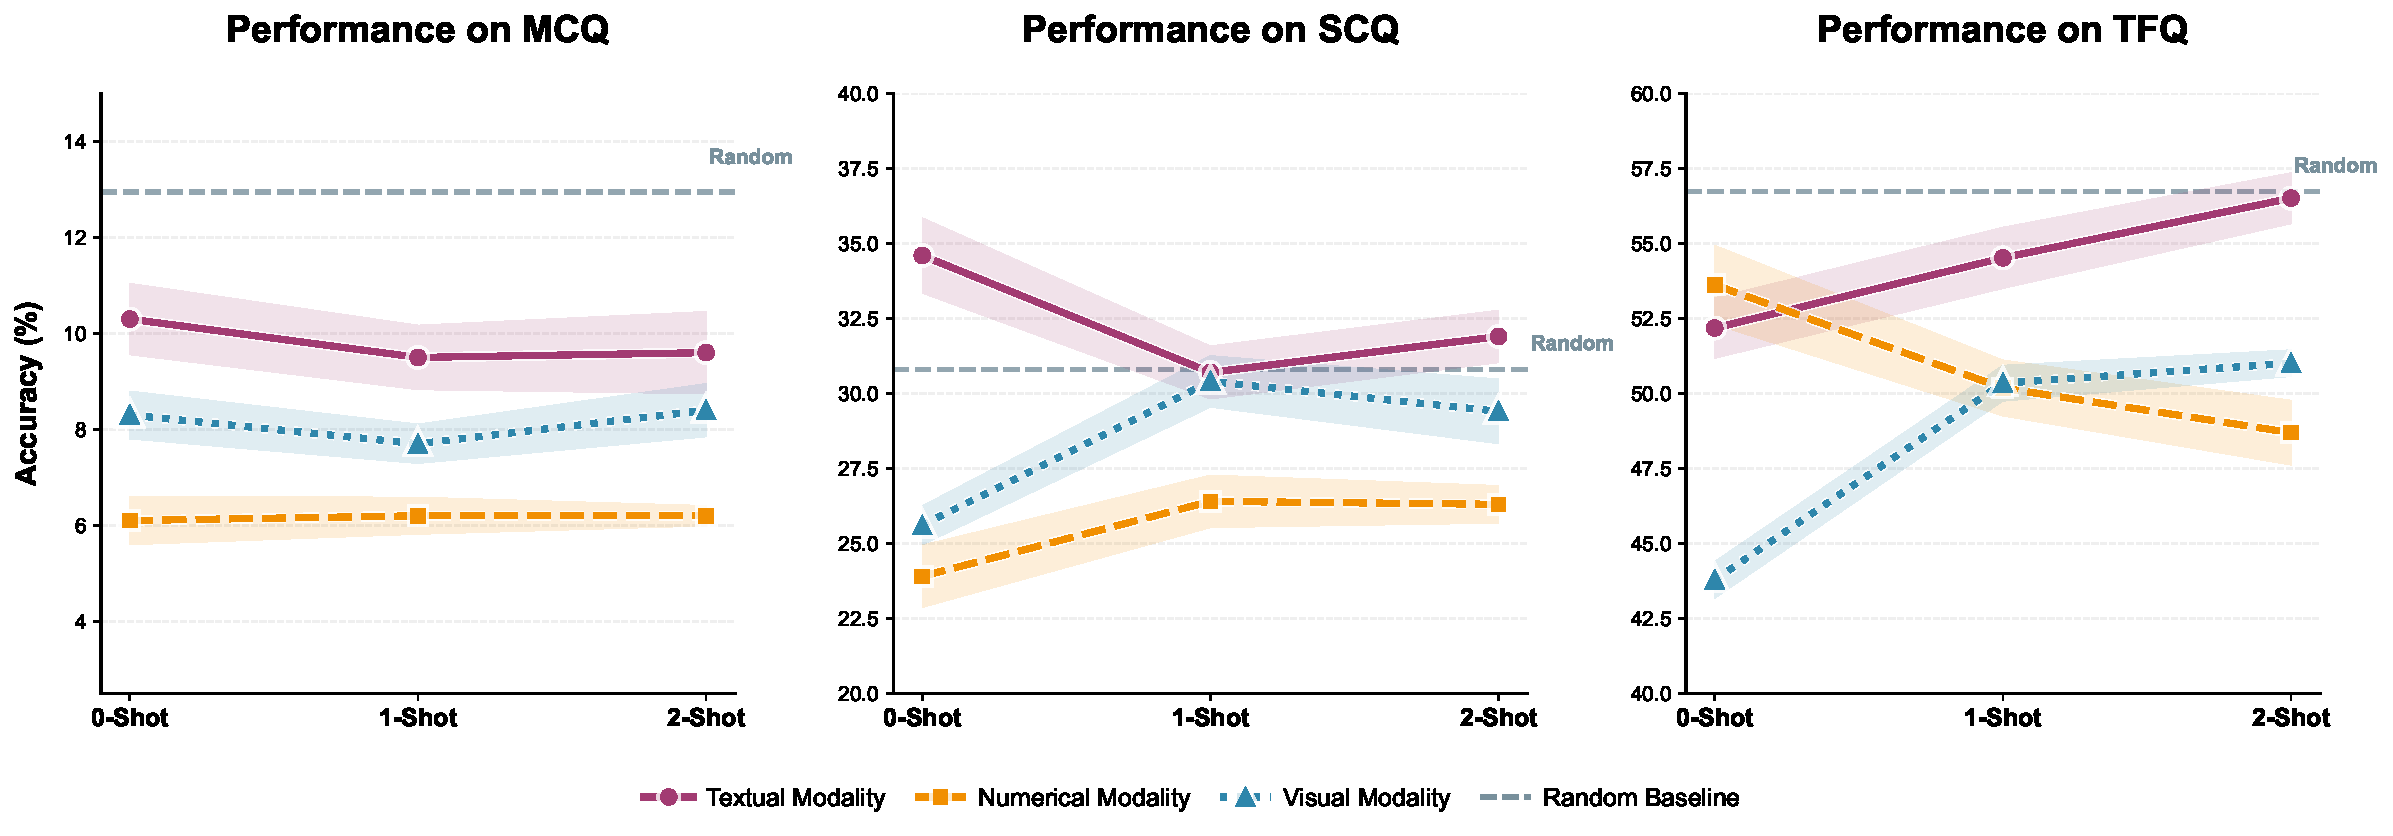
\includegraphics[width=\linewidth]{figure/figure8.pdf}
	\caption{Few-Shot Learning (FSL) Stress-Test. Accuracy trajectories across 0, 1, and 2-shot settings. Flat or degrading performance near random baselines indicates that FSL fails to trigger endogenous cognitive reasoning.}
	\label{fig:few_shot_ablation}
\end{figure*}

\subsection{High-Level Cognition}
\label{HLC}

To gain deeper insight into the cognitive bottlenecks of High-Level Cognition for LLMs, we decompose each incorrect response by identifying its most probable point of failure within the U/S/R pipeline across modalities in Figure ~\ref{fig:HCL}, following the criteria detailed in Appendix~\ref{sec:usrules}. 

This diagnostic perspective serves as a vital complement to holistic accuracy: it reveals that models with comparable performance may nonetheless exhibit fundamentally distinct failure modes, exposing unique fractures along their internal cognitive chains. 
In the \emph{textual} modality, the majority of errors ($65.5\%$) are concentrated in the Reasoning stage. 
This suggests that while LLMs can maintain a facade of Understanding by adhering to output constraints (low U-fail), they lack the underlying world model to execute correct physical deduction. 
Meanwhile, as we shift to the \emph{numerical} and \emph{visual} modalities, we observe a surge in U-fail (reaching $46.7\%$ in visual tasks). 
This indicates that raw physical signals act as representational noise that disrupts the models' instruction-following stability, causing them to abandon the requested output formats entirely. 
Furthermore, the high S-fail in the \emph{numerical} modality ($31.8\%$) reflects a profound internal logical dissonance, where models simultaneously generate mutually exclusive physical states. 

These findings suggest that the next frontier for LLM research is not merely improving answer accuracy, but building models whose \textbf{cognitive pipelines remain structurally coherent} even when reasoning must emerge directly from raw world signals rather than semantic shortcuts.


\subsection{Open-Ended Evolution}
\label{evolution}
Facing specific physical-world problems, the training process of the model essentially serves as a mechanism to approximate the performance upper bound for a given task.

Empirical results in Figure ~\ref{fig:evolution} demonstrate that traditional architecture models establish a stable performance baseline through training, representing the physical upper bound of the \emph{passive fitting} capacity on specific data distributions within traditional AI paradigms. 
However, a compelling phenomenon emerges: 
despite undergoing equivalent training regimes, LLMs not only fail to surpass but comprehensively underperform compared to traditional architecture models. 
This performance therefore inversion exposes profound architectural limitations within LLMs: 
they are fundamentally incapable of efficiently achieving passive fitting to specific physical dynamics, even within closed environments. 

Following an a fortiori argument, Open-ended Evolution requires an intelligent agent to \textbf{continuously assimilate and reorganize knowledge} through active interaction with complex physical environments. 
If current LLMs fail even to reach the upper bound of passive fitting in closed settings, then their limitation is not merely insufficient training, but a more fundamental mismatch between next-token prediction and genuine cognitive evolution. 


\subsection{Exploration and Future Work}
\label{future}

To investigate whether the observed collapse partially stems from the lack of task-specific context, we conducted a rigorous stress-test using \textbf{Few-Shot Learning} (FSL) with 1-shot and 2-shot demonstrations. 
The empirical results reveal a profound stagnation in capability emergence. Despite providing explicit examples, model performance remains stubbornly tethered to the mathematical random baseline. 
% In the numerical modality, for instance, MCQ accuracy remained virtually frozen at approximately $6.20\%$. Most strikingly, in the textual modality, increasing demonstrations to 2-shot actually led to a marginal performance decline (from $10.30\%$ to $9.60\%$). 
Qualitative analysis of the error logs also confirms that while FSL marginally improves template compliance and reducing Understanding-fail pattern, it still fails to trigger any substantive reduction in Reasoning-fail pattern with exacerbated reasoning errors. 
TO summarize, this decoupling proves that FSL in current LLMs provides only \textbf{surface-level alignment} instead of perceiving the underlying laws of the physical world. 

Taken together, the failures across \textbf{modality, cognition, and evolution} indicate that current LLMs are constrained not by missing examples, but by a \emph{paradigm that remains fundamentally text-bound, externally scaffolded, and passively optimized}. 
The next stage of AGI will therefore require a shift from scaling semantic prediction to building systems that can \emph{form unified world representations, maintain endogenous cognitive structure, and grow through real interaction}. 
Under this view, HWI defines a broader transition for the field: from language competence toward authentic world intelligence.

% In the absence of genuine physical logic, additional context acts as "semantic noise" that further destabilizes the model’s fragile reasoning. 
% This decoupling proves that FSL in current LLMs provides only surface-level alignment; it teaches the model how to output a response without enabling the structural cognitive required to perceive the underlying laws of the physical world. 
% Consequently, the persistence of sub-random performance across all shot settings exposes an insurmountable capability ceiling within the "autoregressive next-token prediction" paradigm. 
% These findings demonstrate that AGI cannot be realized through prompt engineering or scaling context alone; it necessitates a paradigm shift toward an endogenous, modality-agnostic architecture capable of autonomous, world-oriented synthesis.
